\documentclass[10pt,a4paper]{article}
\usepackage[utf8]{inputenc}
\usepackage{amsmath}
\usepackage{amsfonts}
\usepackage{amssymb}
\usepackage[]{algorithm2e}
\usepackage{graphicx}
\begin{document}

\title{LINGI2261: Artificial Intelligence \\
Assignement 1 : Solving Problems with Uninformed Search - Numberlink Project}
\author{Ndizera Eddy \and El Jilali Solaiman}
\date{\today}
\maketitle

\section*{Introduction}

\section{Python AIMA}

Here are the answers to the questions regarding the AIMA library.

\begin{enumerate}
	\item \textbf{In order to perform a search, what are the classes that you must define or extend ? Explain precisely why and where they are used inside a tree\_search.} \\

	
	In order to perform a search, the \textbf{Problem} class must be defined. We'll have to implement the following 3 methods  \textit{init}, \textit{goal\_test} and \textit{successor}. \\
	To explain why and where they are used inside a tree\_search, i'll use the pseudocode for a tree\_search (found in IA: a modern approach).\\
	
		
\begin{figure}[!h] %on ouvre l'environnement figure
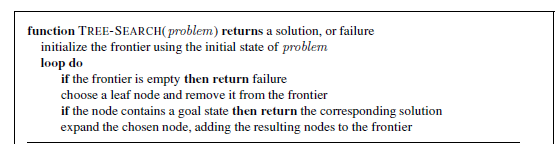
\includegraphics{Tree-Search.png} %ou image.png, .jpeg etc.
\caption{Tree-Search from \textit{Artificial Intelligence a Modern Approach}} %la légende
\label{image_soleil} %l'étiquette pour faire référence à cette image
\end{figure} %on ferme l'environnement figure 
	
	In the pseudocode at the line 1, we see that to initialize we need the initial state of the problem. This initial state is given by the \textit{init} method found in the \textit{Problem} class.\\
	At line 5 of the same pseudocode, to know if we reach the goal, the \textit{goal\_test} method should be called to know that.\\
	Finally, the method \textit{successor} isn't called directly in the pseudocode given. It is called in the \textbf{Node} class by the method\textit{expand} to know the set of children of a given node.\\
	
	All other methods and class in the AIMA library are already well defined.
	%Need to add the pseudocode or snapshots of the aima library to show where it's needed. 
	
	\item \textbf{In the expand method of the class Node what is the advantage of using a yield instead of building a list and returning it afterwards?} \\
	
	The advantage of using a yield is memory usage. By using a yield rather than a list we save space. In the method expand, when we iterate over the list of children of node, we removed them also.\\
	Moreover, in python yield operator allows us to perform lazily. Indeed the call to the lazy operator do only one thing: returning a generator object that will be call later. It allows us to give out new values on the fly and to save memory space
	
	
	\item \textbf{Both breadth\_first\_graph\_search and depth\_first\_graph\_search are matking a call to the same function. How is their fundamental difference implemented?} \\
	
	The fundamental difference between the two functions is the type of queue that they put as parameter when calling the function \textit{graph\_search}.\\
	The first one (breadth) put as queue a \textit{FIFOQueue} whereas the second one (depth) use a \textit{Stack} \textit{LIFOQueue}.\\
	With a \textit{LIFOQueue} the last most recently generated node is chosen for expansion. It implies that we explore first completely a branch before passing to another according to the definition of depth first tree search \\
	With a \textit {FIFOQueue} the first generated node is chosen for expansion. It implies that  we explore first all the nodes of a specific depth according to the definition of breadth first tree search
	
	%Should explain more ?
	
	\item \textbf{What is the difference between the implementation of the graph\_search and the tree\_search methods and how does it impact the search methods?}\\
	
	The difference between the tree\_search and the graph\_search is the variable closed that is a data structures that stocks the nodes already visited. With that we can avoid the infinite loop problem (occuring in depth\_first). 
	
	\item \textbf{What kind of structure is used to implement the closed list? What are the methods involved in the search of an element inside it? What properties must thus have the elements that you can put inside the closed list ?} \\
	
	The closed list is implemented using a dictionnary.\\
	It uses a key to search a value in it. So any element is stored as a key-value pair. The key is like an index in the dictionnary and the value, the element stored.\\
	%Ajouter les methodes/propriété necessaires à un dictionnaire?
	
	The elements must be comparable?, unique?, immutable?.
	
	\item \textbf{How technically can you use the implementation of the closed list to deal with symmetrical states ? }\\
	
	By modifying the compare method of the type used as key as two symmetrical states are equal we can deal with it.
		
\end{enumerate}

\section{The Numberlink Problem}

\begin{enumerate}
	
	\item \textbf{ Explain the advantages and weaknesses of the following search strategies on this problem (not in general): depth first, breadth first.} \\
	
	The depth first search in general takes less time than the breadth first one. Also in this particular problem, the depth first has the completness property like the breadth first because there cannot have infinite search (the square can be filled). \\
	
	For the space occupied by the two serach algorithm, this is not a issue because we use a yield to expand a node and not a list. \\
	
	The breadth first is advantageous with trees that have a high branching factor.
	
	\item \textbf{How can we exploit the uniqueness of solution to reduce the search space? Why is the method pathExists useful?} \\
	
	The method pathExists is useful to know if a a current node don't give an answer. 
	
	\item \textbf{Is the order in which we choose the paths important? How can we use this to reduce the search space? When starting a new path, we can choose to start with any of its two endpoint. How should this choice be done?} \\
	
	Yes it's important. Depending of the order, we can reduce the search space. For that, let's use the example case in your assignement pdf, if we take the D path first, we have 4 choices in total. But if we take the A, we have 5 choices. \\
	
	The choice of endpoins is also important because if we take, in the same example, the e path and take the e point located at the top-right corner, we only have one choice. \\
	
	\item \textbf{What are the advantages and disadvantages of using the tree and graph search for this problem. Which approach would you choose? Which approach allows you to avoid expending twice symmetrical states?} \\
	
	The tree search takes less time in case that the problem cannot have symmetrical states. But the graph search could save time in case symmetrical states are present in the search. \\
	
	The tree search doesn't lose time in checking if the current node has already been visited. Note that this problem cannot have infinite loop (explain why). \\
	
	We will choose the graph search approach. 
	
	\item \textbf{Implement this problem in Python 3. Extend the Problem class and implement the necessary methods and other class(es) if necessary. Your file must be named numberlink.py. You program must take as only input the path to the init file of the problem to solve. It must print to the standard output a solution to the problem satisfying the above format. Your file must be encoded in utf-8. Submit your program on INGInious.} \\
	
	\item \textbf{Experiments must be realized with the 10 instances of the numberlink problem provided. Report in a table the results on the 10 instances for depth-first and breadth- first strategies on both tree and graph search (4 settings). You must report the time, the number of explored nodes and the number of steps from root to solution. When no solution can be found by a strategy in a reasonable time (3 min), explain the reason (time-out and/or swap of the memory). What do you conclude from those experiments?} \\
	

\end{enumerate}

\section*{Conclusion}

\end{document}